\chapter{Contenedores: Docker}
\label{chap:docker}

La primera tecnología que voy a presentar y que he usado en mi proyecto son los contenedores. Comercialmente hablando lleva poco tiempo disponible pero que ha visto un gran incremento inmediato del uso y de la demanda al cubrir muchos aspectos distintos con éxito. Los conceptos independientes que conforman un contenedor, sin embargo, llevan ya bastante tiempo integrados en el kernel de Linux sin haber recibido tanta atención. Empezar por describir esta parte (\ref{sec:cgroups} cgroups) nos llevará a entender mejor otras tecnologías que he usado (Kubernetes) y el ritmo de trabajo que han tenido bajo la tutela de Google.

Los contenedores funcionan en la práctica como una implementación muy ligera de virtualización que nos permite integrar varias aplicaciones independientes sobre una misma máquina sin que se pisen en ningún sentido (ni disco, ni memoria, ni red, ...). Se puede ejecutar de forma reproducible sobre cualquier Linux que tenga una versión del kernel suficientemente actualizada.

\section{Cgroups}
\label{sec:cgroups}

Google empezó a usar tecnología experimental en el kernel de Linux para separar procesos entre sí. En sus clústeres se ejecutan múltiples aplicaciones dentro de la misma máquina\cite{sre2016}, algunas con más prioridad que otras. Se hizo evidente que era necesario algún mecanismo para controlar cuantos recursos gasta cada conjunto de procesos para priorizar los que afectan al usuario y de limitar en caso de error que unas aplicaciones afecten a otras. En 2006 una primera liberación del código que habían usado llegó a Linux bajo el nombre de contenedores\cite{rohitseth2006}, aunque luego se renombraría a grupos de control para evitar confusiones con el término que ya se usaba a nivel de kernel\cite{jonathancorbet2007}. A lo largo del documento usaré \emph{contenedor} para referirme a la implementación de Docker más abstracta, no a este concepto del kernel.

Estos grupos de control clasifican los procesos en ejecución en una jerarquía de namespaces\cite{redhat2016} y permiten aplicar cuotas de control de memoria y otros recursos a dichos grupos. Igualmente podemos decidir que dispositivos son visibles y accesibles para los procesos que tenga dentro.

Se deduce del funcionamiento de cgroups que un cuidadoso protocolo al asignar los namespaces nos conduce directamente a poder separar y controlar los procesos de cada uno de los contenedores en distintos grupos aislándolos entre ellos para conseguir una mayor independencia y control.

Google internamente desarrolló su propia versión de contenedores usando lmctfy\cite{lmctfy} (\emph{Let Me Contain That For You}), aunque nunca llegó a coger la inercia y comunidad de la que Docker disfruta en estos momentos.

\section{Network}
\label{sec:docker-network}

El segundo gran pilar sobre el que se sustenta cualquier virtualización es poder aislar las operaciones de red. Esto permite por ejemplo mantener un mismo mapa de puertos duplicado para cada contenedor para que ambos puedan escuchar en el puerto 80 sin pisarse mutuamente.

Docker implementa este aislamiento de red con un par de interfaces\cite{dockernetworking} unidas por un puente (\emph{bridge}). Una de las interfaces se configura dentro del contenedor y otra se une a una interfaz común a todos \emph{docker0}. La interfaz común \emph{docker0} tiene una IP privada (normalmente 172.17.0.1, aunque depende del sistema y puede configurarse) que pone en comunicación al host con cualquiera de los contenedores siempre que haya alguna aplicación al otro lado del puente escuchando. Podemos ver un gráfico con el diagrama de red en la figura \ref{fig:docker-network}

Esta configuración tiene muchas ventajas más allá del aislamiento:
\begin{itemize}
    \item Podemos escuchar en todas las IPs (0.0.0.0) sin peligros de seguridad, sabemos que ningún atacante externo a la máquina podría llegar jamás a nuestra interfaz de red.
    \item Al tener cada interfaz su mapa de puertos independientes podemos abrir dos servidores en el puerto HTTP 80 por ejemplo, sin que se pisen de ninguna manera.
\end{itemize}

\begin{figure}[H]
    \centering
    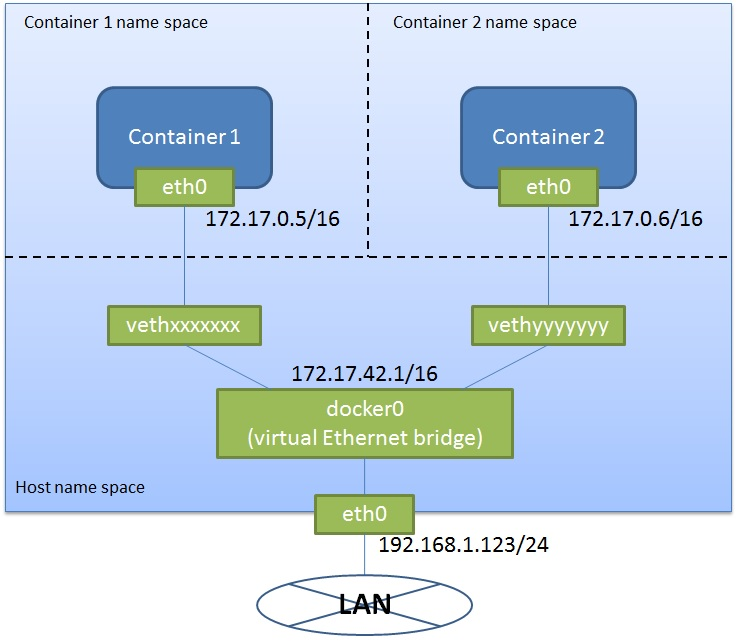
\includegraphics[width=\textwidth]{../images/docker/network.jpg}
    \caption{Diagrama de la red de dos contenedores \protect\cite{kaitoyamada2015}}
    \label{fig:docker-network}
\end{figure}

Implementado el aislamiento se procedió a buscar justamente lo contrario. En algunos casos controlados queremos exponer ciertos puertos al resto de la máquina (o a la red si la máquina está conectada). Cuando ejecutamos un contenedor de Docker podemos decidir asociar algún o algunos puertos internos a otros externos no necesariamente iguales. Podemos por ejemplo exponer los dos contenedores mencionados antes que escuchan en el puerto 80 asociados a los puertos 8081 y 8082 respectivamente sin que ello suponga tener que cambiar nada de la configuración del servidor.

\newpage

Esta flexibilidad de decidir sobre los puertos tiene muchas ventajas:
\begin{itemize}
    \item Podemos dejar alguno de los puertos sin exponer. Por ejemplo publicamos el puerto para que el cliente de MongoDB se conecte, pero no publicamos el puerto de la replicación porque tenemos una sola instancia. Esto reduce los peligros de seguridad en caso de una mala configuración del cortafuegos o un intento de ataque externo de algún tipo.
    \item La asociación de puertos internos y externos se hace a tiempo de ejecución, permitiendo al operador tomar decisiones claves sobre como administrar la máquina y repartir el mapa de puertos común.
    \item Ni el desarrollador ni el operador tienen que cambiar ninguna configuración ni código del contenedor al mover el puerto por el que se accede a un servicio.
\end{itemize}

\section{Ficheros por capas}
\label{sec:ficheros-capas}

El tercer gran pilar necesario para la virtualización es el aislamiento de los ficheros a los que puede acceder el contenedor para que no toque los del host ni los de otros contenedores. Aquí existe un precendente claro que es chroot\cite{linuxchroot}. Esta llamada nos permite cambiar el directorio raíz efectivo que ve el proceso al que llamamos. Docker llegó más allá y no solamente diseñó el sistema para aislar, sino que además lo estableció como solo lectura, una de las grandes ventajas de usar contenedores.

Tanto si usamos AUFS\cite{dockeraufs} como el nuevo driver BRTFS\cite{dockerbtrfs} el funcionamiento externo es el mismo. Se guarda el estado de todo el árbol de ficheros asociado a un hash único a modo de una especie de control de versiones. Cada imagen(ver \ref{sec:docker-images} para más información sobre las imágenes) está formada por varias capas que se construyen una sobre la siguiente sucesivamente. El propio contenedor en ejecución que use esa imagen conforma la última capa que es editable en tanto en cuanto no salgamos del contenedor, que entonces se perdería todo y volvería a tener el estado puro elegido por la imagen en la próxima ejecución.

Se pueden observar las simulitudes y diferencias entre AUFS y BRTFS en las figuras \ref{fig:docker-aufs-layers} y \ref{fig:docker-btrfs-layers}.

\begin{figure}[H]
    \centering
    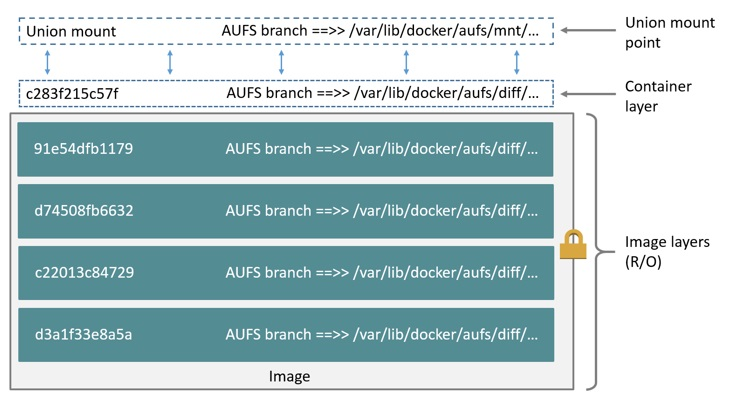
\includegraphics[width=\textwidth]{../images/docker/aufs-layers.jpg}
    \caption{Diagrama de capas en AUFS \protect\cite{dockeraufs}}
    \label{fig:docker-aufs-layers}
\end{figure}

\begin{figure}[H]
    \centering
    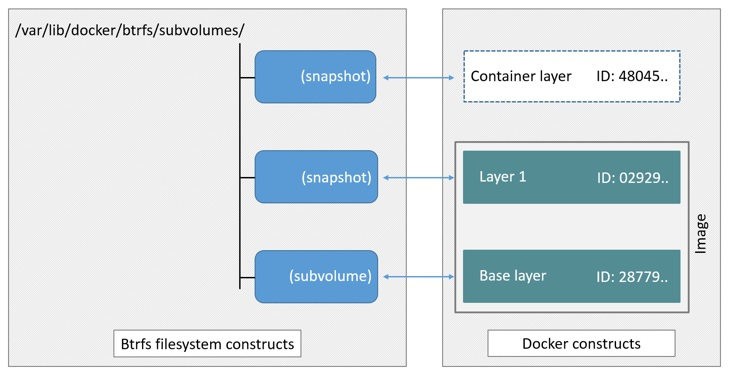
\includegraphics[width=\textwidth]{../images/docker/btrfs-layers.jpg}
    \caption{Diagrama de capas (snapshots) en BTRFS \protect\cite{dockerbtrfs}}
    \label{fig:docker-btrfs-layers}
\end{figure}

Este sistema de ficheros por capas proporciona una ventaja competitiva inmediata a Docker. Algunos usos típicos:
\begin{itemize}
    \item Abrir un contenedor de desarrollo para pruebas. Al cerrarlo no queda nada en la máquina host y se puede empezar de cero con otras pruebas sin romper nada.
    \item Entornos reproducibles para pruebas automatizadas o ejecuciones de software para QA (código reproducible en issues de Github, etc.).
    \item Ficheros temporales de caché que se eliminan al salir del contenedor.
\end{itemize}

Cada capa lleva asociada un hash que la identifica de forma inequívoca. Como las capas son de solo lectura, y cualquier modificación daría lugar a una nueva capa encima de ella con otro hash distinto, podemos evitar descargar o almacenar en disco doblemente el contenido. En la práctica el driver implementa un grafo de relaciones entre las distintas capas para evitar duplicidades en disco. Dicho de otra manera, si dos imágenes A y B contienen 5 capas similares y otras 3/7 distintas respectivamente, en total se guardarán en disco 5 + 3 + 7; las 5 comunes no estarán duplicadas, no supondrán almacenamiento doble. Esto puede aprovecharse para mantener un conjunto estable de imágenes base que se usen en todas las aplicaciones que se pueda que se vayan a ejecutar en un mismo cluster (Debian Jessie con curl instalado, por ejemplo) para optimizar el uso del disco y de la red al encender los contenedores.

\section{Volúmenes}
\label{sec:docker-volumenes}

\subsection{Carpetas del host}
\label{sec:docker-volumen-host}

Dado el sistema de ficheros por capas existe la necesidad de poder configurar puntos de anclaje que hagan que una carpeta del host sea visible y/o editable por el contenedor. Con Docker se pueden configurar a tiempo de ejecución rutas del host que deben asociarse a rutas dentro del sistema de ficheros del contenedor. Estas rutas se montan usando mecanismos típicos de Linux de la misma manera que se procede con un USB o un CD que se inserta en la bandeja del equipo (\emph{mount} y \emph{unmount}).

El uso de los volúmenes puede es bastante flexible, permite:
\begin{itemize}
    \item Montar carpetas de datos para que sobrevivan al período de vida del contenedor. Una base de datos por ejemplo necesita que sus datos permanezcan por siempre.
    \item Montar ficheros donde se estén enviando logs para poder reenviarlos con otro contenedor o desde el host a una localización remota, o simplemente leerlos. Por ejemplo el fichero de acceso de un servidor Apache.
    \item Montar carpetas del sistema para configuraciones avanzadas. Permite por ejemeplo que contenedores como \emph{sysdig}\cite{sysdig} o \emph{cAdvisor}\cite{cadvisor} accedan a datos de monitorización de la máquina.
    \item Montar carpetas comunes entre varios contenedores para compartir datos.
\end{itemize}

\subsection{Otros plugins}
\label{sec:docker-volumen-plugins}

Con el paso del tiempo el sistema de volúmenes ha ido avanzando y ahora mismo se implementa mediante un sistema de plugins. Dicho de otra manera cualquier persona puede implementar un driver que llegue más allá que una simple carpeta del host. Estos plugins unen los contenedores a todo tipo de tecnologías\cite{dockervolumeplugins}, entre las que cabe destacar algunas de ellas:
\begin{itemize}
    \item NFS. Para montar una carpeta situada en alguna localización de la red.
    \item GlusterFS. Un proyecto libre de Red Hat para montar varios servidores como un solo sistema de ficheros compartido y replicado.
    \item GCE/AWS. Crean y unen discos de estas plataformas en la nube en la máquina antes de montar la carpeta.
\end{itemize}

Las especificaciones para escribir tu propio plugin son públicas\cite{dockerwritevolumeplugin} e implementables por cualquier persona en cualquier lenguaje de programación que prefiera.

\section{Imágenes}
\label{sec:docker-images}

Docker permite que se añadan etiquetas (nombres) a una capa concreta. Recordemos que una capa se identifica inequívocamente por un hash, que comprende todo el contenido que lleva dentro. Estos nombres pueden ser más amigables al usuario de cara a que lo teclee por línea de comandos o los escriba en ficheros de configuración.

Por costumbre suele definirse una etiqueta \emph{latest} apuntando a la última imagen construida como punto de referencia; además de otras que queramos definir por número de versión (\emph{ubuntu:14.04}), fecha, nombre (\emph{google:debian}), etc.

Cuando se ejecuta un contenedor podemos especificar el nombre de una imagen para que la use. Como veremos más adelante los nombres de las imágenes tienen significado especial a la hora de compartir públicamente la imagen ya construida usando el registro \ref{sec:docker-registry} y pueden usarse para descargarla justo antes de la ejecución.

Aparte de construir una imagen como veremos en el siguiente apartado a veces hay que empezar de cero para construir algunas imágenes básicas de sistemas operativos. Para ello Docker nos provee de un comando\cite{dockerload} que permite construir imágenes desde un fichero comprimido con todo el contenido que no parte de ninguna capa previa.

\section{Dockerfile}
\label{sec:dockerfile}

Se puede construir una imagen directamente comando a comando y marcando el punto donde queremos que se haga una capa\cite{dockerimagecommit}. Sin embargo esta técnica carece de una reproducción sencilla por otros miembros del equipo, o de poder cambiar un pequeño paso en todo el proceso. Normalmente las imágenes se construyen usando un fichero de configuración denominado \emph{Dockerfile}.

El fichero usa una sintaxis propia\cite{dockerfile} pero fácil de usar. Nos permite por ejemplo especificar la imagen de la que queremos partir, comandos de instalación que queramos ejecutar, ficheros que necesitamos copiar, incluso el programa que se debe abrir al ejecutar el contenedor. Tiene bastantes directivas, algunas de los cuales se usan solo en ocasiones excepcionales, así que prefiero referirme a la documentación oficial para que las explique todos ellos.

\begin{minted}[baselinestretch=1.2]{dockerfile}
FROM golang:1.7
RUN apt-get install curl
COPY fnapi /opt/fnapi
CMD ["/opt/fnapi"]
\end{minted}

Los Dockerfiles tienen la ventaja de ser reproducibles: tan solo tenemos que cambiar el comando concreto que necesitemos y volver a construir la imagen. Además Docker hace uso de las imágenes por capas para empezar la construcción en la capa que haya cambiado, reutilizando el resto. Cada directiva del fichero crea una nueva capa de la imagen, por lo que comúnmente se busca agrupar todos los comandos posibles en la misma.
\begin{minted}[baselinestretch=1.2]{dockerfile}
FROM golang:1.7
RUN apt-get update && \
    apt-get install curl
COPY fnapi /opt/fnapi
CMD ["/opt/fnapi"]
\end{minted}

\section{Docker registry}
\label{sec:docker-registry}

La gran ventaja que ofrece Docker es poder reusar imágenes ya hechas o Dockerfiles ya preparados en tus propias imágenes y Dockerfiles. Esto no es algo nuevo, ya existía software como Chef\cite{chef} o Puppet\cite{puppet} que ofrecen pequeñas recetas hechas por otra gente para usar directamente o adaptar. Docker tuvo desde el principio una buena historia con la comunidad con su Docker Hub\cite{dockerhub} que permitía que cualquier compartiera imágenes y las reusara. Además expone claramente el Dockerfile que es un fichero único y sencillo (a diferencia de Puppet o Chef que suelen tener varios y suele ser programación directamente). Por todo esto me atrevo a decir que el registro online y/o el poder descargarse el registro (en un contenedor, claro) para ejecutarlo en tus servidores han contribuido enormemente al éxito del que disfruta la tecnología de contenedores actualmente.

Para subir una imagen, aparte de registrarla si procede online (no todos lo requieren), simplemente hay que etiquetar con el nombre adecuado y pedirle a Docker que suba los ficheros al registro. Luego cualquier persona con acceso puede descargarlo por esa misma etiqueta para ejecutarla o usarla como base de otra imagen.

\section{Comparaciones con otras tecnologías}
\label{sec:docker-compare}

\subsection{Máquinas virtuales}
\label{subsec:docker-compare-vm}

Las ideas que dan forma a Docker no son nuevas en su mayoría y algunas veces puede parecer que los contenedores funcionan igual que otras tecnologías previas que sin embargo son muy diferentes. Es el caso con las máquinas virtuales. Se puede ejecutar procesos aislados, sistema de ficheros aislados, red aislada, todo se borra al reiniciar, ...; son todas características que también poseen las VM. Sin embargo no hay que olvidar el origen de los contenedores en cgroup para encontrar cuatro diferencias principales.

Primeramente es el kernel el que aísla los procesos. Todos los contenedores de la máquina comparten acceso al kernel, para bien o para mal. No se pueden ejecutar dos kernels distintos, ni por el mismo precio, un kernel de pruebas. Igualmente si algún contenedor consiguiera explotar consciente o inadvertidamente un error puede afectar al resto de contenedores. Por ejemplo una issue que lleva varios años sin solución\cite{tankywoo2014} hace que Docker deje de responder y que haya que reiniciar la máquina para continuar.

Por otra parte aunque podamos instalar o partir de un Ubuntu o un Debian por ejemplo, realmente solo hemos copiado los ficheros que tenían de otras capas, pero no es un sistema operativo funcionando normalmente. No ejecuta crons a menos que le digamos, no se actualiza, no ejecuta ningún script ni instalación, ...; simplemente copia las configuraciones y binarios para que podamos usarlos. A efectos prácticos el resultado suele ser similar pero especialmente el tema de los crons y otros demonios (\emph{logrotate}) puede afectar a usuarios que no conocen esto y no se lo esperan.

Tercero, al necesitar un kernel necesitan por tanto un Linux. Si queremos ejecutar contenedores sobre Windows o Mac necesitamos una máquina virtual real (normalmente \emph{BusyBox} o algo parecido) y tecnología de virtualización real (\emph{VirtualBox}, \emph{VMWare}, ...). Procedemos a ejecutar el demonio dentro de la máquina y el cliente de Docker se puede comunicar a través de la API desde fuera con él para simular el mismo uso que tiene Linux. Esto es lo que implementa Docker Machine\cite{dockermachine} por ejemplo.

Por último aunque se le pueden asignar cuotas a los contenedores, no es como una máquina virtual que tenemos que saber a priori que recursos asignarle. Un contenedor puede llegar a ocupar el 100\% de la CPU o el 100\% de la memoria si queremos. No hay un sobrecoste de ejecutarse sobre una virtualización como en el caso de las VM.

Todo esto nos lleva a afirmar que un contenedor no es una VM\cite{mikecoleman2016} y que tampoco debe administrarse como tal: no debe recibir parches de seguridad, no debe tener un servidor SSH, no deben hacerse backups del software que lleve el contenedor, etc.

\subsection{LXC}
\label{subsec:docker-compare-lxc}

LXC\cite{lxc} da fundamento libre de intereses de empresa a los contenedores en Linux. Sin embargo carece de los aspecto más avanzados y útiles para la comunidad como los Dockerfiles o un registro centralizado y público. Se usa de una forma parecida a Docker: bajándonos imágenes ya hechas y ejecutándolas.

\subsection{Rocket}
\label{subsec:docker-compare-rocker}

Surge en CoreOS como alternativa a la plataforma de Docker\cite{coreosrkt}. La empresa ha ido añadiendo servicios de nube, DNS y otros que no forman parte de los contenedores en sí mismos, todo ello sobre un solo binario monolítico cada vez más grande e inseguro. Rocket intenta volver a la filosofía de Unix de un solo binario que hace un solo trabajo y lo hace bien, huyendo de la arquitectura cliente-servidor de Docker que tantos problemas ha causado con systemd\cite{dockersystemd} y huyendo de la complicación reflejada sobre los usuarios de que cerrar el cliente no para las acciones del servidor. Además lo están implementando con una serie de programas independientes e intercambiables, cada uno con su estándar y todo código abierto y redactado en comunidad; a diferencia de Docker qué redacta sus propios estándares y protocolos en privado. Rocket puede ejecutar imágenes de Docker, incluso puede descargarlas de los registros; aparte de ejecutar su propio formato libre de imágenes para contenedores.

La única razón de no usarlo para el proyecto es que Minikube, la herramienta que uso para encender y experimentar con Kubernetes en el PC local, usa Docker Machine. Como menciono antes Machine usa VirtualBox o similares para preparar una instalación independiente de Docker, sin posibilidad de reemplazarlo por Rocket.

\subsection{lmctfy}
\label{subsec:docker-compare-lmctfy}

Se usa mucho dentro de Google, pero no tiene documentación aceptable ni extensa públicamente. Tampoco disfruta de ningún tipo de Dockerfile ni registro central; y ciertamente los comandos no son directos ni intuitivos porque interactúan directamente con los permisos de cgroups.

Está en buen estado y actualizado pero seguramente es más recomendable usar tecnologías que hayan sido pensadas para el público en general y no basta con que se haya liberado el código de la herramienta.
